% Single-file Overleaf source. All figures are generated in TikZ/PGFPlots; bibliography is embedded below.
\documentclass[conference]{IEEEtran}

\usepackage{cite}

\usepackage{amsmath}

\usepackage{graphicx}

\usepackage{array}

\usepackage{float}

\usepackage{placeins}

\usepackage{listings}

\usepackage{balance}

\usepackage{pgfplots}

\pgfplotsset{compat=1.17}

\usepackage{booktabs}

\usepackage{multirow}

\usepackage{url}

\usepackage{hyperref}

\hypersetup{hidelinks}

\usepackage{tikz}

\usetikzlibrary{matrix,positioning,shapes.geometric,arrows.meta}



\newcolumntype{L}[1]{>{\raggedright\arraybackslash}p{#1}}



\lstset{
    basicstyle=\ttfamily\footnotesize,
    breaklines=true,
    columns=fullflexible,
    frame=single,
    captionpos=b,
    aboveskip=6pt,
    belowskip=6pt,
    showstringspaces=false
}



\title{An Empirical Evaluation of White-Box and Black-Box Testing Techniques for Software Quality Assurance Using Fault Injection}



\author{
\IEEEauthorblockN{Anand Nakum}
\IEEEauthorblockA{Computer Science and Engineering\\
Institute of Technology, Nirma University\\
Ahmedabad, India\\
23bce190@nirmauni.ac.in}
\and
\IEEEauthorblockN{Yagnik Nandasana}
\IEEEauthorblockA{Computer Science and Engineering\\
Institute of Technology, Nirma University\\
Ahmedabad, India\\
23bce192@nirmauni.ac.in}
}



\begin{document}

\raggedbottom

\maketitle



%----------------------------------------------------------------------

\begin{abstract}

Software testing is an integral part of the Software Development Life Cycle (SDLC). It plays a significant role in the final quality of the software product.

This paper contains the results of a controlled experiment to compare the effectiveness of five test-design techniques: statement coverage, branch coverage, decision-table testing, orthogonal array testing (OAT), and a combination of these with the addition of some boundary-value test cases. These were applied to a common E-commerce Discount System written in Python.

Using a seeded-fault harness with eight manually encoded mutants (M1-M8), the ability of each suite to achieve high statement and branch coverage on the correct system implementation (10 ~statements, 6~branch outcomes) and its fault-detection capability were evaluated.

Each of the five test suites managed to attain 100\% statement and branch coverage on the correct implementation. The four baseline suites managed to detect six out of eight faults (75\% detection rate), while the hybrid suite, with the addition of two test cases reaching the 5000-unit threshold, achieved an impressive 100\% detection rate.

The two faults not detected by the baseline suites (M1 and M8) were both related to the threshold, requiring test inputs to reach or surpass it to trigger them.

The conclusion is that while full structural coverage does not ensure fault detection, adding a few test cases with values close to the threshold can greatly improve detection capability in some cases. The results are specific to the eight faults and the one system tested but provide some justification for hybrid approaches to testing. The results do not indicate that such approaches are universally superior.
\end{abstract}



\begin{IEEEkeywords}

White-box testing, Black-box testing, Fault injection, Seeded-fault experiment, Boundary-value testing, Hybrid testing, Software quality assurance

\end{IEEEkeywords}



%----------------------------------------------------------------------

\section{Introduction}

\label{sec:intro}



The role of software testing in the Software Development Life Cycle (SDLC) is very important because it affects the quality, reliability and correctness of software systems~\cite{nidhra2012,izzat2023}.

With the growth of software size and complexity testing has become an ever growing and important process for defect prevention, risk reduction and overall software quality assurance (SQA).



The goal of testing extends beyond just detecting defects

It helps to verify and validate software and to decrease the effort spent on software maintenance and increase the confidence in the software system implemented to meet functional and structural expectations~\cite{kumar2015}.

Of the many testing methods available, white-box testing and black-box testing are the two most basic and popular methods~\cite{nidhra2012,alshamaa2025}.

The white-box testing concentrates on the internal logic and control flow of a program, whereas black-box testing is all about what the program does, based on requirements and expectations of the users.

Each of these techniques addresses a different dimension of quality that can't be completely covered by the other approaches, so using only one technique for assurance is rarely adequate~\cite{maspupah2025}.



SQA is traditionally judged on the effectiveness of the testing techniques, traditionally by their ability to detect seeded or real faults, and structural coverage (e.g. statement and branch coverage)~\cite{jia2011}.

Coverage metrics represent the percentage of code covered by testing, but not directly measure the fault-detection capability.

An alternative form of evaluation is available, and known as fault injection, which deliberately introduces known faults into the program and explicitly measures the capacity of a test suite to detect correct and faulty behavior~\cite{jia2011}.



This paper reviews two families of test sets and applies them to a test set of the same E-commerce Discount System, a function that maps three data characteristics (purchase amount, membership status, and coupon availability) to a discount amount, requiring a decision.

First, four different basic test-design techniques, one hybrid suite, and structural coverage are applied to the correct implementation.

Next, we perform a seeded-fault experiment with eight manually encoded faults (M1-M8) to compare the fault-detection rates for the five suites.



The remainder of this paper is organized as follows.

Section~\ref{sec:litreview} reviews related work.

Section~\ref{sec:gap} identifies the research gap and states the research questions.

Section~\ref{sec:whitebox} and Section~\ref{sec:blackbox} describe white-box and black-box testing, respectively, as applied to the case-study system.

Section~\ref{sec:methodology} presents the experimental methodology, including the fault model and metrics.

Section~\ref{sec:results} reports the results.

Section~\ref{sec:comparison} compares the testing techniques.

Section~\ref{sec:discussion} discusses the findings.

Section~\ref{sec:threats} addresses threats to validity.

Section~\ref{sec:conclusion} concludes the paper and outlines future work.





%----------------------------------------------------------------------

\section{Literature Review}

\label{sec:litreview}



There are many software testing techniques which are studied, specifically with regard to white-box and black-box software testing.



Nidhra and Dondeti~\cite{nidhra2012} provide a comprehensive review of both types of test families, and finally conclude that white-box testing methods are suitable to identify logical errors while black-box testing methods can be used for identifying functional requirements.



Kumar et al.~\cite{kumar2015} have explained that white-box testing is mostly appropriate in the unit testing phase of software testing while black-box testing is suitable at the system and acceptance testing phase of software testing.



Maspupah~\cite{maspupah2025} studied the pros and cons of both testing types and found that, the more the testing types used, the more chances of having a defect detected and the better the overall quality of the software product.



Izzat and Saleem~\cite{izzat2023} analysed various software testing techniques and tools, and emphasized the need of software automation and systematics in software test case generation.



AbuSalim et al.~\cite{abuslim2021} have investigated the software testing techniques in the area of mobile application and discussed its applicability in real-life scenarios, both white and black-box testing.



Alshamaa and Saleem~\cite{alshamaa2025} made an overview of the most important black-box testing techniques and found that the selection of the testing technique should depend on the testing objectives, required resources and the ability to find system faults.



Jalal et al.~\cite{jalal2026} proposed a method that uses machine learning techniques to ease the process of improvement of black box testing.



Jia and Harman~\cite{jia2011} present a comprehensive review of mutation testing, in which artificial faults (also known as mutants) are inserted in a program to test the effectiveness of a test suite in detecting faults in the program.

They have pointed out that the mutation score is the most important characteristic of this ability, and that the equivalent mutants and high computational requirements are the difficulties.

Although we use seeded faults in our experiment which are prescribed manually, rather than using mutation operators, the fundamental concept of measuring the capability of tests to discriminate between faulty and correct behavior remains the same.

Overall, the references mentioned here demonstrate that white-box and black-box testing are complementary and not conflicting.

However, the cited literature is limited to general surveys or specific comparisons of different testing approaches, with only a few controlled experiments that compare multiple testing approaches applied to the same system and under the same specific conditions, e.g., by providing the same fault-injection metrics.



Table~\ref{tab:litreview} summarizes the cited literature.



\begin{table*}[!t]

\centering

\caption{Summary of literature review}

\label{tab:litreview}

\begin{tabular}{|c|L{2.4cm}|L{4.0cm}|c|L{2.8cm}|L{3.8cm}|}
\hline
\textbf{Ref.} & \textbf{Authors} & \textbf{Title} & \textbf{Year} & \textbf{Focus} & \textbf{Key Findings} \\
\hline
\cite{nidhra2012} & S.~Nidhra, J.~Dondeti & Black Box and White Box Testing Techniques: A Literature Review & 2012 & Comparative review & Establishes distinction between structural and functional testing. \\
\hline
\cite{kumar2015} & M.~Kumar et al. & A Comparative Study of Black Box Testing and White Box Testing Techniques & 2015 & Testing techniques and SDLC phases & White-box for unit testing; black-box for system/acceptance testing. \\
\hline
\cite{abuslim2021} & S.~W.~G.~AbuSalim et al. & Comparative Analysis of Software Testing Techniques for Mobile Applications & 2021 & Mobile testing & Practical relevance of testing techniques in real environments. \\
\hline
\cite{izzat2023} & S.~K.~Izzat, N.~N.~Saleem & Software Testing Techniques and Tools: A Review & 2023 & Methods, path analysis, tools & Systematic design and automation improve testing efficiency. \\
\hline
\cite{maspupah2025} & A.~Maspupah & Literature Review: Advantages and Disadvantages of Black Box and White Box Testing Methods & 2025 & Strengths and limitations & Combining both families improves defect detection. \\
\hline
\cite{alshamaa2025} & Z.~M.~Alshamaa, N.~N.~Saleem & Black Box Software Testing Techniques: A Literature Review & 2025 & Black-box selection criteria & Technique selection should depend on goals, effort, and fault detection. \\
\hline
\cite{jalal2026} & H.~N.~Jalal et al. & Enhancing Black Box Testing Through Machine Learning Techniques & 2026 & AI-driven test prioritization & ML improves scalability and testing efficiency. \\
\hline
\cite{jia2011} & Y.~Jia, M.~Harman & An Analysis and Survey of the Development of Mutation Testing & 2011 & Mutation testing survey & Defines mutation score; discusses equivalent mutants and cost. \\
\hline
\end{tabular}

\end{table*}





%----------------------------------------------------------------------

\section{Research Gap, Questions, and Contributions}

\label{sec:gap}



White-box and black-box testing methods have been studied in great detail in the past, but most analyses compare or evaluate the methods in isolation.

There have been few efforts to merge various test-design methods into a single test system, and reliability evaluation of the various methods using controlled fault injection has been limited.

In addition, it is often suggested that structural and functional testing methods should be incorporated and this is not always shown with quantitative evidence from a seeded-fault experiment.



This inspires the present study whose research questions are:



\begin{itemize}

    \item \textbf{RQ1:} How do the selected white-box and black-box test suites compare in detecting the eight seeded faults in the E-commerce Discount System?

    \item \textbf{RQ2:} What is the impact of including boundary-value cases in the hybrid suite for this case study?

    \item \textbf{RQ3:} Are the ability to cover statements and branches sufficient for these test suites to find the seeded faults?

    \item \textbf{RQ4:} What is the trade-off between the size of the test suite and the effectiveness of the seeded faults for this experiment?

\end{itemize}



\noindent\textbf{Contributions.}

We present a carefully chosen comparison of four well-known test-design methods as well as an extended hybrid suite, based on the same discount method, identical coverage measure, a quantitative comparison of the number of tests and detection rate, and eight documented seeded faults.

This study does not measure all aspects of software product quality, such as the aspects defined in the ISO/IEC~25010; it aims to study the effectiveness of software testing and the ability to detect defects during software testing~\cite{iso25010}.





%----------------------------------------------------------------------

\section{White-Box Testing}

\label{sec:whitebox}



White-box testing is a method of testing by which the internal logic, structure, conditions and execution paths are analyzed of the software.

Test cases should be designed by the tester who should know the source code and design of the program.


It's a technique that is frequently applied during unit testing, integration testing and code level verification~\cite{nidhra2012,kumar2015}.



\subsection{Advantages}

\begin{itemize}

\item Identifies logical errors and programming errors.

\item Enhances code quality by running internal paths.

\item Allows coverage of structures to be measured (statement, branch).

\item Detects dead code, unused paths and hidden faults.

\item Is very practical during unit level testing.

\end{itemize}



\subsection{Disadvantages}

\begin{itemize}

\item Knows programming and internal structure.

\item May not be able to identify the missing requirements and functional gaps.

\item Can be complicated and time consuming in large software systems.

\item It requires a lot of the implementation details; any changes in code may necessitate changes to test cases.

\end{itemize}



\subsection{System Under Test}

\label{sec:sut}

This paper provides a sample E-commerce Discount System throughout, for both white-box and black-box testing purposes.

The program takes as input the amount purchased, and the availability of a discount coupon as well as the membership.

The business rules are:



\begin{itemize}

\item If \texttt{amount} $\geq$ 5000 and the customer is a member, discount = 20\% of amount.

\item If \texttt{amount} $\geq$ 5000 and the customer is not a member, discount = 10\% of amount.

\item If \texttt{amount} $<$ 5000 and a coupon is available, discount = 500.

\item If \texttt{amount} $<$ 5000 and no coupon is available, discount = 0.

\end{itemize}



The reference implementation is written in Python (Listing~\ref{lst:discount_py}) and resides in \texttt{src/discount\_system.py}.

It is exercised by five test suites located in the \texttt{tests/} directory.



\begin{lstlisting}[language=Python,caption={Python implementation of the discount calculation},label={lst:discount_py}]
def calculate_discount(amount, is_member,
                       has_coupon):
    discount = 0.0
    if amount >= 5000:
        if is_member == 1:
            discount = amount * 0.20
        else:
            discount = amount * 0.10
    else:
        if has_coupon == 1:
            discount = 500.0
        else:
            discount = 0.0
    return discount
\end{lstlisting}



\subsection{Flowchart}

Figure~\ref{fig:flowchart} presents the processing logic of the discount program.

The flow begins with input collection, checks whether the amount is $\geq$~5000, and then proceeds to either the membership decision or the coupon decision before returning the final discount.



\begin{figure}[!t]

\centering

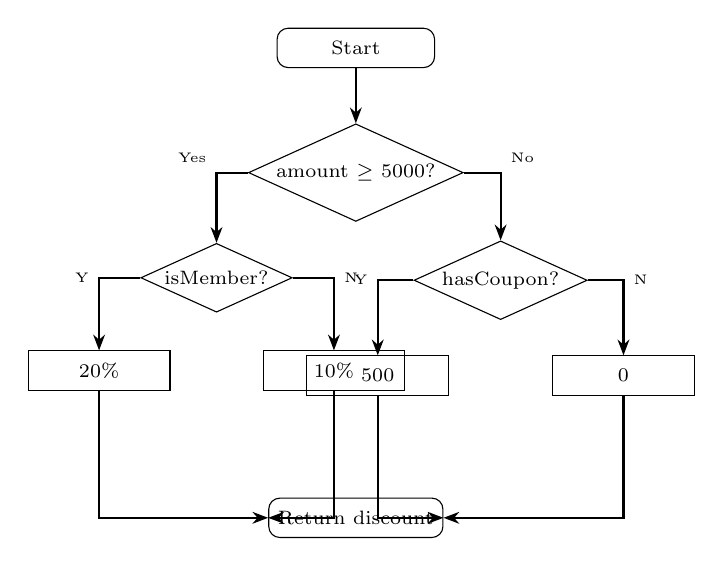
\begin{tikzpicture}[
  node distance=0.7cm,
  startstop/.style={rectangle, rounded corners, draw, minimum width=2cm, minimum height=0.5cm, font=\scriptsize},
  decision/.style={diamond, draw, aspect=2.2, minimum width=1cm, font=\scriptsize, inner sep=1pt},
  process/.style={rectangle, draw, minimum width=1.8cm, minimum height=0.5cm, font=\scriptsize},
  arrow/.style={-{Stealth[length=2mm]}, thick}
]
\node (start) [startstop] {Start};
\node (d1) [decision, below=of start] {amount $\geq$ 5000?};
\node (d2) [decision, below left=0.8cm and 0.6cm of d1] {isMember?};
\node (d3) [decision, below right=0.8cm and 0.6cm of d1] {hasCoupon?};
\node (p1) [process, below left=0.7cm and 0.1cm of d2] {20\%};
\node (p2) [process, below right=0.7cm and 0.1cm of d2] {10\%};
\node (p3) [process, below left=0.7cm and 0.1cm of d3] {500};
\node (p4) [process, below right=0.7cm and 0.1cm of d3] {0};
\node (ret) [startstop, below=3.5cm of d1] {Return discount};
\draw [arrow] (start) -- (d1);
\draw [arrow] (d1) -| node[above left, font=\tiny]{Yes} (d2);
\draw [arrow] (d1) -| node[above right, font=\tiny]{No} (d3);
\draw [arrow] (d2) -| node[left, font=\tiny]{Y} (p1);
\draw [arrow] (d2) -| node[right, font=\tiny]{N} (p2);
\draw [arrow] (d3) -| node[left, font=\tiny]{Y} (p3);
\draw [arrow] (d3) -| node[right, font=\tiny]{N} (p4);
\draw [arrow] (p1) |- (ret);
\draw [arrow] (p2) |- (ret);
\draw [arrow] (p3) |- (ret);
\draw [arrow] (p4) |- (ret);
\end{tikzpicture}

\caption{Program flowchart of the E-commerce Discount System.}

\label{fig:flowchart}

\end{figure}



\subsection{Cyclomatic Complexity}

The discount logic contains three decision points: the amount check, the membership check, and the coupon check.

The cyclomatic complexity of the program is $V(G) = 3 + 1 = 4$, indicating four linearly independent paths through the control flow.

This explains why four carefully selected test cases are sufficient to exercise all independent structural paths in this case study.



\subsection{Method~1: Branch Coverage}

White-box testing is one type of branch coverage which is a method that all branches in the program must be traversed at least once~\cite{nidhra2012}.

This is crucial in the discount program, as the outcome relies on the nested if-else statement.

Branch coverage checks the correctness of the outcomes of the three decisions, both true and false.



The relevant decision conditions are:

\begin{itemize}

\item \texttt{amount} $\geq$ 5000

\item \texttt{isMember} == 1

\item \texttt{hasCoupon} == 1

\end{itemize}



To achieve complete branch coverage, test cases must force each of these decisions to evaluate to both True and False.

The four required logical routes are:

(1)~amount=True, member=True;

(2)~amount=True, member=False;

(3)~amount=False, coupon=True;

(4)~amount=False, coupon=False.



Table~\ref{tab:branch_tc} shows the test cases for branch coverage.



\begin{table}[!t]

\centering

\caption{Test cases for branch coverage}

\label{tab:branch_tc}

\begin{tabular}{|c|c|c|c|}
\hline
\textbf{TC} & \textbf{Input} & \textbf{Branches} & \textbf{Expected} \\
\hline
TC1 & (8000, 1, 0) & amt=T, mem=T & 1600 \\
TC2 & (8000, 0, 0) & amt=T, mem=F & 800 \\
TC3 & (3000, 0, 1) & amt=F, cpn=T & 500 \\
TC4 & (3000, 1, 0) & amt=F, cpn=F & 0 \\
\hline
\end{tabular}

\end{table}



Each of the decision branches are exercised in the program is covered, which means that all the possible outcomes of the nested control structure are exercised.

This gives you better proof than running through all statements once that the logic is correct.



\subsection{Method~2: Statement Coverage}

Statement Coverage - All executable statements in the program are run at least once~\cite{nidhra2012}.

It does not need to find every possible path taken, but it does need to find a path that allows each statement in the code to be executed.



The corresponding execution paths are:

\begin{itemize}

\item Path~1: $A \to B(T) \to C(T) \to D \to I$

\item Path~2: $A \to B(T) \to C(F) \to E \to I$

\item Path~3: $A \to B(F) \to F(T) \to G \to I$

\item Path~4: $A \to B(F) \to F(F) \to H \to I$

\end{itemize}



Table~\ref{tab:stmt_tc} shows the test cases for statement coverage.



\begin{table}[!t]

\centering

\caption{Test cases for statement coverage}

\label{tab:stmt_tc}

\begin{tabular}{|c|c|c|c|}
\hline
\textbf{TC} & \textbf{Input} & \textbf{Path} & \textbf{Expected} \\
\hline
TC1 & (8000, 1, 0) & A-B-C-D-I & 1600 \\
TC2 & (8000, 0, 0) & A-B-C-E-I & 800 \\
TC3 & (3000, 0, 1) & A-B-F-G-I & 500 \\
TC4 & (3000, 1, 0) & A-B-F-H-I & 0 \\
\hline
\end{tabular}

\end{table}



For this program, the same four inputs are used for branch coverage as well, and therefore they are also used for statement coverage, since each of the statements is on a different decision controlled path.

This effect comes from the compactness of the selected discount logic and cannot be extrapolated to larger systems.




%----------------------------------------------------------------------

\section{Black-Box Testing}

\label{sec:blackbox}



Black-box testing is a type of functional testing that is used to test the functionality of software without any reference to its internal structure or source code.

The tester tests the input-output behavior; checks if the system meets the required input-output behavior~\cite{nidhra2012,alshamaa2025}.



\subsection{Advantages}

\begin{itemize}

\item Does not need programming skills or source code to access.

\item Useful for determining the function and user expectations.

\item Identifies the absence of features and interface issues.

\item Can be used by independent testers from the user point of view.

\item Good for system testing and acceptance testing.

\end{itemize}



\subsection{Disadvantages}

\begin{itemize}

\item Does not offer any understanding of the structure of the internal code.

\item May be unable to detect logical errors in the implementation.

\item May need a lot of input combinations to provide complete coverage.

\item Is unable to directly measure the internal code coverage.

\end{itemize}



\subsection{Method~1: Decision Table Testing}

Decision Table Testing is a black-box method used when system behavior can be described as a set of conditions and actions~\cite{alshamaa2025,maspupah2025}.

The discount problem is well suited because the output is determined by explicit business rules.



The decision table uses the following conditions and actions:

\begin{itemize}

\item C1: Amount $\geq$ 5000 \quad\quad A1: Apply 20\% discount

\item C2: User is a member \quad\quad A2: Apply 10\% discount

\item C3: Coupon available \quad\quad A3: Apply 500 discount

\item \hfill A4: No discount

\end{itemize}



When the amount is $\geq$~5000, the coupon condition is irrelevant because the program directly selects a percentage discount based solely on membership status.



Table~\ref{tab:decision_table} shows the decision table, and Table~\ref{tab:dt_tc} the corresponding test cases.



\begin{table}[!t]

\centering

\caption{Decision table for the discount system}

\label{tab:decision_table}

\begin{tabular}{|c|c|c|c|c|}
\hline
\textbf{Rule} & \textbf{C1} & \textbf{C2} & \textbf{C3} & \textbf{Action} \\
\hline
R1 & Yes & Yes & -- & A1 (20\%) \\
R2 & Yes & No & -- & A2 (10\%) \\
R3 & No & -- & Yes & A3 (500) \\
R4 & No & -- & No & A4 (0) \\
\hline
\end{tabular}

\end{table}



\begin{table}[!t]

\centering

\caption{Test cases using decision table testing}

\label{tab:dt_tc}

\begin{tabular}{|c|c|c|c|}
\hline
\textbf{TC} & \textbf{Input} & \textbf{Rule} & \textbf{Expected} \\
\hline
TC1 & (8000, 1, 0) & R1 & 1600 \\
TC2 & (8000, 0, 1) & R2 & 800 \\
TC3 & (3000, 0, 1) & R3 & 500 \\
TC4 & (3000, 1, 0) & R4 & 0 \\
\hline
\end{tabular}

\end{table}



There is a correct mapping of each functional rule to the output that is expected, proving that the technique is very useful for validating business-rule logic.



\subsection{Method~2: Orthogonal Array Testing (OAT)}

OAT is a black-box technique to limit the number of test cases while ensuring that significant interactions between parameters are being tested~\cite{izzat2023,jalal2026}.

The goal of OAT is to pick a subset of the possible combinations that has pairwise coverage without testing all combinations.



For the discount system, the parameters are:

\begin{itemize}

\item P1: Purchase amount $\to \{<5000, \geq 5000\}$.

\item P2: Membership $\to \{\text{Member}, \text{Non-Member}\}$.

\item P3: Coupon availability $\to \{\text{Yes}, \text{No}\}$.

\end{itemize}



Because there are three factors that are each at two levels, an L4 orthogonal arrangement is adequate.

The total possible combinations are $2 \times 2 \times 2 = 8$; OAT reduces them to four representative cases (50\% reduction).

This decrease is only observed in this small system and should not be extrapolated to larger systems without additional supporting data.



Table~\ref{tab:oat_array} and Table~\ref{tab:oat_tc} show the L4 array and corresponding test cases.



\begin{table}[!t]

\centering

\caption{L4 orthogonal array for the discount system}

\label{tab:oat_array}

\begin{tabular}{|c|c|c|c|}
\hline
\textbf{TC} & \textbf{Amount} & \textbf{Member} & \textbf{Coupon} \\
\hline
TC1 & $\geq$5000 & Member & Yes \\
TC2 & $\geq$5000 & Non-Member & No \\
TC3 & $<$5000 & Member & No \\
TC4 & $<$5000 & Non-Member & Yes \\
\hline
\end{tabular}

\end{table}



\begin{table}[!t]

\centering

\caption{Test cases using OAT}

\label{tab:oat_tc}

\begin{tabular}{|c|c|c|}
\hline
\textbf{TC} & \textbf{Input} & \textbf{Expected} \\
\hline
TC1 & (8000, Member, Yes) & 1600 \\
TC2 & (8000, Non-Mem, No) & 800 \\
TC3 & (3000, Member, No) & 0 \\
TC4 & (3000, Non-Mem, Yes) & 500 \\
\hline
\end{tabular}

\end{table}





%----------------------------------------------------------------------

\section{Experimental Methodology}

\label{sec:methodology}



\subsection{Overview}

This experiment uses a controlled seeded-fault (fault-injection) approach to compare the fault-detection effectiveness of five test suites on the E-commerce Discount System.

Does not call upon an automated mutation testing engine, such as PIT or MutPy.

Rather, it takes the burden of manually defining eight faulty implementations in the script \texttt{run\_experiment.py}.


All the faulty variants change exactly one portion of the discount logic and the experiment measures the detection capabilities of each test suite for the seeded faults.



\subsection{Test Suites}

\label{sec:suites}

Four baseline suites each contain four test cases.

The hybrid suite adds four boundary-value cases (at amounts 4999 and 5000), resulting in eight test cases.

Table~\ref{tab:testcases} summarizes the suite sizes.



\begin{table}[!t]

\centering

\caption{Number of test cases per suite}

\label{tab:testcases}

\begin{tabular}{|l|c|}
\hline
\textbf{Suite} & \textbf{Test cases} \\
\hline
Statement Coverage & 4 \\
Branch Coverage & 4 \\
Decision Table & 4 \\
OAT & 4 \\
Hybrid + boundary & 8 \\
\hline
\textbf{Total} & \textbf{24} \\
\hline
\end{tabular}

\end{table}



The statement-coverage and branch-coverage suites have the same four input combinations as the original paper's design;

this is because the four cases are required for 100\% statement and branch coverage with a compact structure of the discount function.

As they use the same set of input images, the fact that they do not yield the same set of fault detections would be surprising and, therefore, would not be interpreted as evidence of a general difference (or equivalence) between these two techniques.



\subsection{Fault Model}

\label{sec:mutants}

The eight seeded faults (M1--M8) are listed in Table~\ref{tab:mutants}.

Each mutant modifies the discount logic in a single, specific way.



\begin{table}[!t]

\centering

\caption{Seeded faults (M1--M8) in the discount system}

\label{tab:mutants}

\begin{tabular}{|c|L{5.8cm}|}
\hline
\textbf{ID} & \textbf{Description} \\
\hline
M1 & Change \texttt{amount >= 5000} to \texttt{amount > 5000} (relational operator) \\
M2 & Invert the membership condition (\texttt{is\_member == 1} $\to$ \texttt{is\_member == 0}) \\
M3 & Change member discount rate from 20\% to 30\% \\
M4 & Change non-member discount rate from 10\% to 15\% \\
M5 & Reverse the coupon condition (\texttt{has\_coupon == 1} $\to$ \texttt{has\_coupon == 0}) \\
M6 & Change flat coupon discount from 500 to 50 \\
M7 & Change no-coupon result from 0 to 100 \\
M8 & Shift threshold from 5000 to 6000 \\
\hline
\end{tabular}

\end{table}



These faults are deliberately selected to represent common fault categories: relational-operator replacement (M1), condition negation (M2, M5), constant replacement (M3, M4, M6, M7), and threshold shift (M8).

They are not a random or statistically representative sample of all possible real-world defects.



\subsection{Experimental Execution}

\label{sec:execution}

The experiment proceeds as follows:

\begin{enumerate}

\item Run all 24 functional tests against the correct reference implementation using \texttt{pytest}~\cite{pytest2026} to confirm all pass.

\item Measure statement and branch coverage for each suite individually using \texttt{coverage.py}~\cite{coverage2026} with the \texttt{-{}-branch} option.

\item For each suite and each mutant, execute all test cases against the faulty implementation and record whether any test produces an output differing from the expected result.

A fault is \emph{detected} (killed) if at least one test case produces a discrepant output; it \emph{survives} otherwise.

\item Aggregate results into the CSV file \texttt{results/fault\_injection\_results.csv}.

\end{enumerate}



\subsection{Metrics}

\label{sec:metrics}

We report the following metrics:



\begin{itemize}

\item \textbf{Statement coverage (\%):} Percentage of executable statements exercised by the test suite on the correct implementation.

\item \textbf{Branch coverage (\%):} Percentage of decision outcomes exercised.

\item \textbf{Fault-detection rate (\%):} Defined as:

\end{itemize}



\begin{equation}
\text{Fault-detection rate} = \frac{\text{Faults detected}}{\text{Faults injected}} \times 100
\label{eq:fdr}
\end{equation}



For this experiment there are eight injected faults.

A surviving fault is a fault that was not detected by the test inputs in this suite, but does not mean that the fault is harmless throughout the universe.




%----------------------------------------------------------------------

\section{Results}

\label{sec:results}



\subsection{Test Execution}

Passes all 24 functional tests against the correct implementation on Python ($\texttt{py -m pytest -q}$: 24~passed).



\subsection{Coverage}

100\% statement coverage (10/10~statements) and 100\% branch coverage (6/6~branch outcomes) is obtained for all five suites on the correct implementation.

Each of the suites was individually covered by running \texttt{coverage.py} with the \texttt{-{}-branch} flag.



\subsection{Fault-Detection Results}

Table~\ref{tab:exp_results} presents the complete experimental results, verified against the CSV output of \texttt{run\_experiment.py}.



\begin{table*}[!t]

\centering

\caption{Experimental results: coverage and fault detection for eight seeded faults}

\label{tab:exp_results}

\begin{tabular}{|l|c|c|c|c|c|c|c|}
\hline
\textbf{Suite} & \textbf{Test cases} & \textbf{Stmt cov.} & \textbf{Branch cov.} & \textbf{Killed} & \textbf{Survived} & \textbf{Detection rate} & \textbf{Killed mutants} \\
\hline
Statement Coverage & 4 & 100\% & 100\% & 6 & 2 & 75\% & M2--M7 \\
Branch Coverage    & 4 & 100\% & 100\% & 6 & 2 & 75\% & M2--M7 \\
Decision Table     & 4 & 100\% & 100\% & 6 & 2 & 75\% & M2--M7 \\
OAT                & 4 & 100\% & 100\% & 6 & 2 & 75\% & M2--M7 \\
Hybrid + boundary  & 8 & 100\% & 100\% & 8 & 0 & 100\% & M1--M8 \\
\hline
\end{tabular}

\end{table*}



\subsection{Fault-Detection Rate Comparison}

Figure~\ref{fig:bar_chart} visualizes the fault-detection rates for the five suites.



%----------------------------------------------------------
% Fault-Detection Rate Comparison — Full-Width Horizontal Chart
%----------------------------------------------------------
\begin{figure*}[!t]
\centering
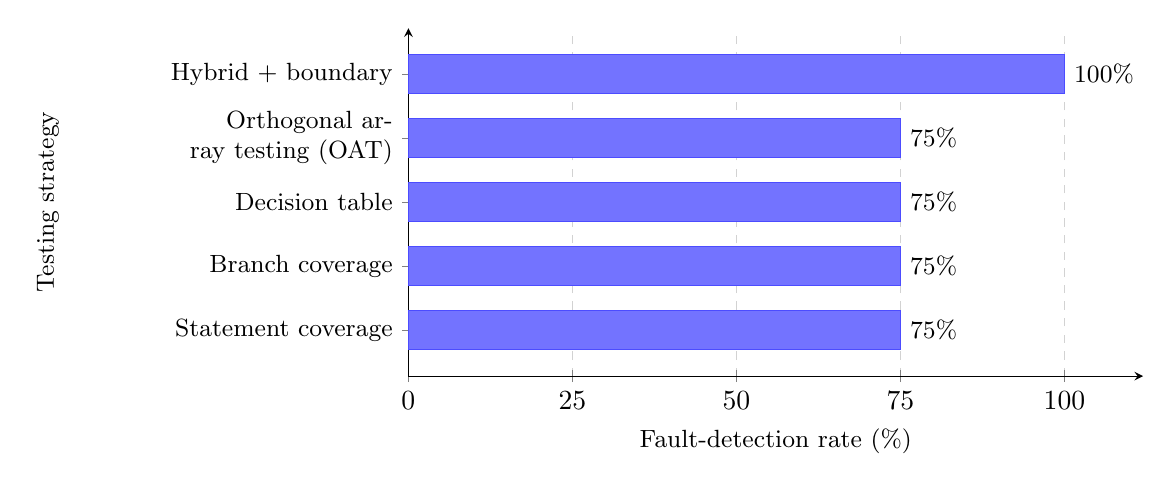
\begin{tikzpicture}
\begin{axis}[
    xbar,
    width=0.90\textwidth,
    height=6.0cm,
    xmin=0,
    xmax=112,
    xlabel={Fault-detection rate (\%)},
    ylabel={Testing strategy},
    symbolic y coords={stmt,branch,decision,oat,hybrid},
    ytick=data,
    yticklabels={
        Statement coverage,
        Branch coverage,
        Decision table,
        Orthogonal array testing (OAT),
        Hybrid + boundary
    },
    yticklabel style={
        font=\small,
        text width=4.0cm,
        align=right
    },
    xlabel style={font=\small},
    ylabel style={font=\small},
    xtick={0,25,50,75,100},
    xmajorgrids=true,
    grid style={dashed,gray!35},
    axis lines=left,
    bar width=14pt,
    enlarge y limits=0.18,
    nodes near coords={
        \pgfmathprintnumber[fixed,precision=0]{\pgfplotspointmeta}\%
    },
    point meta=x,
    every node near coord/.append style={
        font=\small,
        anchor=west
    },
    clip=false
]
\addplot[
    fill=blue!55,
    draw=blue!70
] coordinates {
    (75,stmt)
    (75,branch)
    (75,decision)
    (75,oat)
    (100,hybrid)
};
\end{axis}
\end{tikzpicture}
\caption{Fault-detection rate of five testing strategies across
eight seeded faults. Each baseline suite detects six faults (75\%),
while the hybrid suite with boundary-value cases detects all eight
(100\%).}
\label{fig:bar_chart}
\end{figure*}



\subsection{Mutant-Outcome Matrix}

Table~\ref{tab:mutant_matrix} provides a per-mutant breakdown showing which faults each suite detected (K~=~killed) or missed (S~=~survived).



\begin{table}[!t]

\centering

\caption{Mutant-outcome matrix (K = killed, S = survived)}

\label{tab:mutant_matrix}

\begin{tabular}{|c|c|c|c|c|c|}
\hline
\textbf{Mutant} & \textbf{Stmt} & \textbf{Branch} & \textbf{Dec.T} & \textbf{OAT} & \textbf{Hybrid} \\
\hline
M1 & S & S & S & S & K \\
M2 & K & K & K & K & K \\
M3 & K & K & K & K & K \\
M4 & K & K & K & K & K \\
M5 & K & K & K & K & K \\
M6 & K & K & K & K & K \\
M7 & K & K & K & K & K \\
M8 & S & S & S & S & K \\
\hline
\end{tabular}

\end{table}





%----------------------------------------------------------------------

\section{Comparative Study of Testing Techniques}

\label{sec:comparison}



Table~\ref{tab:comparison} summarizes the strengths and roles of the four testing techniques applied to the discount system.



\begin{table*}[!t]

\centering

\caption{Comparison of testing techniques for the E-commerce Discount System}

\label{tab:comparison}

\begin{tabular}{|L{2.2cm}|L{3cm}|L{3cm}|L{3cm}|L{3cm}|}
\hline
\textbf{Criteria} & \textbf{Statement Coverage} & \textbf{Branch Coverage} & \textbf{Decision Table} & \textbf{OAT} \\
\hline
Approach & White-box & White-box & Black-box & Black-box \\
\hline
Testing basis & Executable statements & Decision outcomes & Functional rules and actions & Input-parameter combinations \\
\hline
Main objective & Execute each statement at least once & Exercise each decision outcome & Validate rule-action correctness & Reduce combinations while retaining pairwise coverage \\
\hline
Strength & Confirms execution of discount actions & Verifies correctness of nested decision logic & Maps directly to discount policy rules & Covers factor interactions with fewer tests \\
\hline
Limitation & Weaker for logic errors & Requires source code knowledge & Can grow when conditions increase & May miss uncommon interaction defects \\
\hline
\end{tabular}

\end{table*}



Branch Coverage and Statement Coverage look at the internal logic.

The two are equal in providing coverage in the sense that both test the true and the false branches of the critical decisions, but Branch Coverage offers more structural assurance.

This particular program both techniques require four identical test cases due to the compact nested structure.

Decision Table testing and OAT focus on the outside function.

Decision Table Testing is the most closely related to the business requirements as it produces a direct mapping between the rules specified and the outputs that are expected.

OAT makes emphasis on efficiency, by reducing the test set.





%----------------------------------------------------------------------

\section{Discussion}

\label{sec:discussion}



\subsection{Coverage vs.\ Fault Detection}

All five suites are 100\% statement and branch covered on the reference implementation, though four of the baseline suites only identify 6 of 8 seeded faults (75\%);


This result directly addresses \textbf{RQ3}: full structural coverage does not guarantee that all seeded faults will be detected.

The coverage measures represent the measure of what code paths have been covered–but they do not guarantee that the test oracle will return a different value for faulty implementations.



\subsection{Threshold-Related Faults}

The remaining faults are all threshold-related: There, fault M1 changes the sign of \texttt{>=} to \texttt{>} and fault M8 changes the threshold from 5000 to 6000.

The amounts 3000 and 8000 are used in the four baseline suites, and are well away from the boundary of 5000 (neither M1 nor M8 produces a discrepant output for those inputs).

The hybrid suite includes test cases for 5000 (at threshold) and 4999 (just below threshold); these reveal both faults.

Adding boundary-value cases at the critical threshold helped to detect the two threshold-related faults in this case study, which answers \textbf{RQ2}.




\subsection{Suite Size Trade-Off}

The hybrid suite includes twice as many test cases as the four (2x), and finds two new fault cases related to the thresholds;

A 25\% improvement (75\% to 100\%) was observed, with a double increase in the number of test cases, which answers \textbf{RQ4}: the improvement was achieved at the expense of doubling test cases.

For larger systems with many parameters the effort would have to be re-evaluated, but in this small example it is not that much.



\subsection{Identical Baseline Scores}

All four base suites have the same base score of 75\%.

The statement-coverage and branch-coverage suites are both identical, by design, so the fact that they reach the same results does not imply a general difference or equivalence between the two techniques.

The decision-table and OAT suites have slightly different combinations of inputs (e.g., different amount of coupons on the high-amount case) but the input combinations in both suites don't reach the 5000 boundary and they also do not hit M1 or M8.



\subsection{Answering RQ1}

This experiment tests the four baseline test-design approaches and finds that all six faults (M2--M7) are detected, and that the hybrid suite, which is extended with boundary-value cases, detects all eight faults.

The above is evidence that the boundary value test design approach is suitable to complement both the structural and functional test design approach to this system and should not be generalized to all systems or all fault distributions.



\subsection{SQA Perspective}

This case study examines one aspect of software quality assurance—the ability of test suites to detect seeded faults (defect detection).

It is not a measure of the other quality aspects specified by the standards, such as ISO/IEC~25010~\cite{iso25010}: performance efficiency, usability, security or maintainability.

The results support testing and verification dimension of SQA by showing that coverage is not enough to measure the effectiveness of testing, and targeted test-design augmentation can enhance detection of defects.





%----------------------------------------------------------------------

\section{Threats to Validity}

\label{sec:threats}



\begin{itemize}

\item \textbf{External validity}: This research employed only one, small discount calculation function.

The findings might not be applicable to larger and more complex software systems.



\item \textbf{Fault-selection validity:} Only eight faults, deliberately designed and manually encoded, were used in this study.

They are no actual defects nor a statistically representative sample of actual defects.



\item \textbf{Construct validity:} Fault detection is defined as a test giving an output that differs from the expected one.

It doesn't reflect the quality of software or all possible failure modes.


\item \textbf{Test-suite comparability:} The statement- and branch-coverage suites were the same with four identical input sets (so they could not be compared).

Do not make comparisons between labels.


\item \textbf{Implementation validity:} Mutants are not automatically generated by a mutation testing tool, rather by hand in the form of Python functions.

This eliminated the computation cost of automated mutation, but reduced the fault coverage to only the eight selected variants.



\item \textbf{Performance validity:} No timing or developer-effort study was performed.

The results do not imply any claims about elapsed time or labor savings.



\item \textbf{Oracle validity:} Expected outputs are in accordance with the given discount rules.

The conclusions are based on the rules that are accurate to the requirements that are intended.
\end{itemize}





%----------------------------------------------------------------------

\section{Conclusion and Future Work}

\label{sec:conclusion}



This paper provided an empirical controlled case study to compare five test design techniques: statement coverage, branch coverage, decision table testing, orthogonal array testing, and a hybrid of the suite of tests with boundary value testing cases, on a case of E-commerce Discount System.

Seeded fault experiment using 8 different manually encoded faulty variants (M1-M8) was applied for the evaluation of structural coverage and fault detection effectiveness.



Key findings:

\begin{itemize}

\item All 5 suites cover 100\% statement and branch coverage of the correct implementation.

\item The four baseline suites detect 6 out of the 8 faults (75\% detection rate) with the remaining 2 faults that are threshold related (M1 and M8).

\item The hybrid suite (8 test cases instead of 4) detects all eight faults (100\% detection rate).

\item Full coverage does not provide fault detection; targeted boundary value testing provides fault detection for the selected faults.

\end{itemize}



The study shows that structural coverage measures are useful, but are not adequate measures of fault detection capability.

The addition of targeted boundary-value tests can dramatically improve detection without adding too many tests, although this will hold true for only the eight seeded faults and one system tested.

Future work will include larger rule-based systems, use automated mutant generation (such as using mutation-testing tools), and evaluate the scalability of hybrid testing strategies for various application domains.



\balance



\begin{thebibliography}{00}

\bibitem{nidhra2012}
S. Nidhra and J. Dondeti, ``Black Box and White Box Testing Techniques---A Literature Review,'' \emph{International Journal of Embedded Systems and Applications}, vol. 2, no. 2, pp. 29--50, 2012, doi: 10.5121/ijesa.2012.2204.

\bibitem{izzat2023}
S. K. Izzat and N. N. Saleem, ``Software Testing Techniques and Tools: A Review,'' \emph{Journal of Education and Science}, vol. 32, no. 2, pp. 30--44, 2023, doi: 10.33899/edusj.2023.137480.1305.

\bibitem{kumar2015}
M. Kumar, S. K. Singh, and R. K. Dwivedi, ``A Comparative Study of Black Box Testing and White Box Testing Techniques,'' \emph{International Journal of Advance Research in Computer Science and Management Studies}, vol. 3, no. 10, 2015.

\bibitem{alshamaa2025}
Z. M. Alshamaa and N. N. Saleem, ``Black Box Software Testing Techniques: A Literature Review,'' \emph{Passer Journal of Basic and Applied Sciences}, vol. 7, no. 2, pp. 1001--1011, 2025, doi: 10.24271/PSR.2025.508216.1963.

\bibitem{maspupah2025}
A. Maspupah, ``Literature Review: Advantages and Disadvantages of Black Box and White Box Testing Methods,'' \emph{Techno Nusa Mandiri: Journal of Computing and Information Technology}, vol. 21, no. 2, pp. 151--162, 2025, doi: 10.33480/techno.v21i2.5776.

\bibitem{abuslim2021}
S. W. G. AbuSalim, R. Ibrahim, and J. A. Wahab, ``Comparative Analysis of Software Testing Techniques for Mobile Applications,'' \emph{Journal of Physics: Conference Series}, vol. 1793, no. 1, Art. no. 012036, 2021, doi: 10.1088/1742-6596/1793/1/012036.

\bibitem{jalal2026}
H. N. Jalal, A. Alhroob, A. Shaheen, and W. Alzyadat, ``Exploring Diverse Perspectives: Enhancing Black Box Testing Through Machine Learning Techniques,'' \emph{International Journal of Informatics and Communication Technology}, vol. 15, no. 1, pp. 238--246, 2026, doi: 10.11591/ijict.v15i1.pp238-246.

\bibitem{jia2011}
Y. Jia and M. Harman, ``An Analysis and Survey of the Development of Mutation Testing,'' \emph{IEEE Transactions on Software Engineering}, vol. 37, no. 5, pp. 649--678, 2011, doi: 10.1109/TSE.2010.62.

\bibitem{iso25010}
ISO/IEC, \emph{ISO/IEC 25010:2023: Systems and Software Engineering---Systems and Software Quality Requirements and Evaluation (SQuaRE)---Product Quality Model}, 2nd ed., 2023. [Online]. Available: \url{https://www.iso.org/standard/78176.html}

\bibitem{pytest2026}
pytest Development Team, ``pytest Documentation: Get Started.'' [Online]. Available: \url{https://docs.pytest.org/en/latest/getting-started.html}. Accessed: Oct. 22, 2026.

\bibitem{coverage2026}
Coverage.py Development Team, ``coverage.py Documentation.'' [Online]. Available: \url{https://coverage.readthedocs.io/en/latest/}. Accessed: Oct. 22, 2026.

\end{thebibliography}

\end{document}